%%%%%%%%%%%%%%%%%%%%%%%%%%%%%%%%%%%%%%%%%%%%%%%%%%%%%%%%%
%%             东南大学数电实验报告 LaTeX 模板
%%                SEU-Circuit-Report.cls
%% https://github.com/Teddy-van-Jerry/SEU_Digital_Report
%% ======================================================
%% 版本信息:
%% v1.0 (Nov. 07, 2021)
%% ------------------------------------------------------
%% 模板制作:
%% Teddy van Jerry, (me@teddy-van-jerry.org)
%% * GitHub: https://github.com/Teddy-van-Jerry
%% * Website: https://teddy-van-jerry.org
%% * Blog: https://blog.teddy-van-jerry.org
%% ------------------------------------------------------
%% 使用说明:
%% 1. 编译使用 XeLaTeX 和 Biber
%% 2. 报告基本信息通过修改导言区以 exp 开头的命令
%% 3. 参考文献位于 ref/ref.bib
%% 4. 报告模板依据 MIT License 开源共享
%% ------------------------------------------------------
%% Copyright 2021 (c) Teddy van Jerry
%%
%% Permission is hereby granted, free of charge, to any
%% person obtaining a copy of this software and
%% associated documentation files (the "Software"), to
%% deal in the Software without restriction, including
%% without limitation the rights to use, copy, modify,
%% merge, publish, distribute, sublicense, and/or sell
%% copies of the Software, and to permit persons to whom
%% the Software is furnished to do so, subject to the
%% following conditions:
%%
%% The above copyright notice and this permission notice
%% shall be included in all copies or substantial
%% portions of the Software.
%% 
%% THE SOFTWARE IS PROVIDED "AS IS", WITHOUT WARRANTY OF
%% ANY KIND, EXPRESS OR IMPLIED, INCLUDING BUT NOT
%% LIMITED TO THE WARRANTIES OF MERCHANTABILITY, FITNESS
%% FOR A PARTICULAR PURPOSE AND NONINFRINGEMENT. IN NO
%% EVENT SHALL THE AUTHORS OR COPYRIGHT HOLDERS BE LIABLE
%% FOR ANY CLAIM, DAMAGES OR OTHER LIABILITY, WHETHER IN
%% AN ACTION OF CONTRACT, TORT OR OTHERWISE, ARISING
%% FROM, OUT OF OR IN CONNECTION WITH THE SOFTWARE OR THE
%% USE OR OTHER DEALINGS IN THE SOFTWARE.
%%%%%%%%%%%%%%%%%%%%%%%%%%%%%%%%%%%%%%%%%%%%%%%%%%%%%%%%%%

%% 使用实验报告模板类(字体大小 11pt 约为五号字)
\documentclass[fontset=windows,11pt]{SEU-Digital-Report}

%%%%%%%%%%%%%%%%%%%% 报告基本信息 %%%%%%%%%%%%%%%%%%%%
\expno{一} % 实验序号
\expname{数据传送} % 实验名称
\expauthor{薛宇飞 } % 姓名
\expID{04020235} % 学号
\expmates{} % 同组
\expmatesID{} % 学号(同组)
\expmajor{信息工程} % 专业
\explab{金智楼硬件实验室} % 实验室
\expdate{\today} % 实验日期
\expreportdate{\today} % 实验日期
\expgrade{} % 成绩评定
\exptutor{裴文江} % 评阅教师
%%%%%%%%%%%%%%%%%%%%%%%%%%%%%%%%%%%%%%%%%%%%%%%%%%%%
\usepackage{xeCJK}
\usepackage{threeparttable} %table添加注释
\usepackage{colortbl}
\newcommand{\grayrow}{\rowcolor[rgb]{ .906, .902, .902}}
\usepackage{pgfplots}
\pgfplotsset{compat=1.11}

%% 报告正文
\begin{document}

% 打印封面页
\exptitlepage

\tableofcontents
\newpage

\section{实验目的与内容}       
\begin{enumerate}
    \item 熟悉 8086 指令系统的数据传送指令,进一步掌握传送指令的寻址方式;
    \item 利用 \texttt{Turbo Debugger} 调试工具来调试汇编程序。   
\end{enumerate}














% 打印参考文献
\addcontentsline{toc}{section}{参考文献}
\printbibliography

\end{document}


%%%%%%%%%%%%%%%%%%%%%%%%%%%%%%%%%%%%%%%%%%%%%%%%%%%%%%%%

% 序号段落样例
\begin{enumerate}
    \item 熟悉数字逻辑与硬件接口基本实验仪器(双踪数字示波器、双路波形发生器等)的使用;   
\end{enumerate}

% 表格样例
\begin{table}[htbp]
    \centering
    \caption{Parameters for the simulation \label{tab:parameters}}
    \bgroup\def\arraystretch{1.5}
    \setlength{\tabcolsep}{4.5mm}
      \begin{threeparttable}%要写注释,得加这行
        \begin{tabular}{c|c}
          \toprule
          \textbf{Parameter} & \textbf{Value}\\
          \midrule\midrule
          \grayrow $(M,\,N),\,(M_G,\,N_G)$,\,$(L_G,\,L_h)$ & (64, 32),\,(100, 32),\,(3, 3)\\
          $(\lambda,\, n_t)$ & $\left(5\, \text{mm} ,\, \mathcal{C} \mathcal{N} (0, P^2_n)\right)$\\
          \grayrow $\vartheta$, $\gamma$ and $\phi $ & $\mathtt{rand}\ [-\frac{\pi}{2}, \frac{\pi}{2}]$\\ 
          \bottomrule
        \end{tabular}
        %注释
        \begin{tablenotes}%注释开始
        \footnotesize
        \item[$\ast$] $\mathtt{rand}\ [a, b]\ (a<b)$ is a random value generated between $a$ and $b$.
        \end{tablenotes}%注释结束
      \end{threeparttable}%要写注释,得加这行
    \egroup
  \end{table}

% 并排两张图样例
\begin{figure}[htbp]
    \centering
    \subfloat[原理图]{
        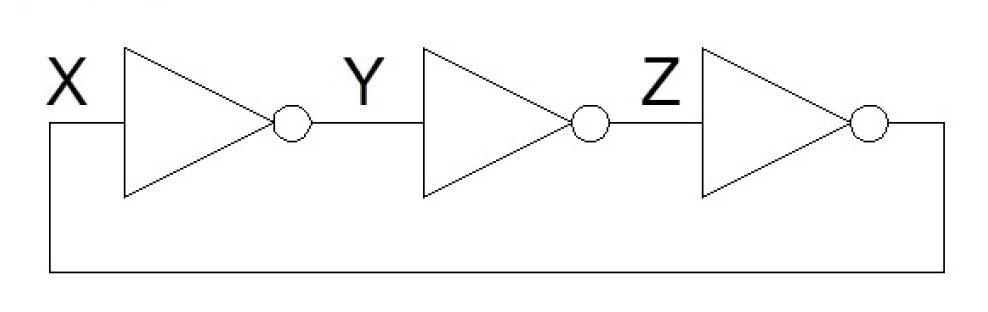
\includegraphics[height=2cm]{fig/oscillation_init.png}
        \label{subfig:oscillation_init}
    }
    \subfloat[等效图]{
        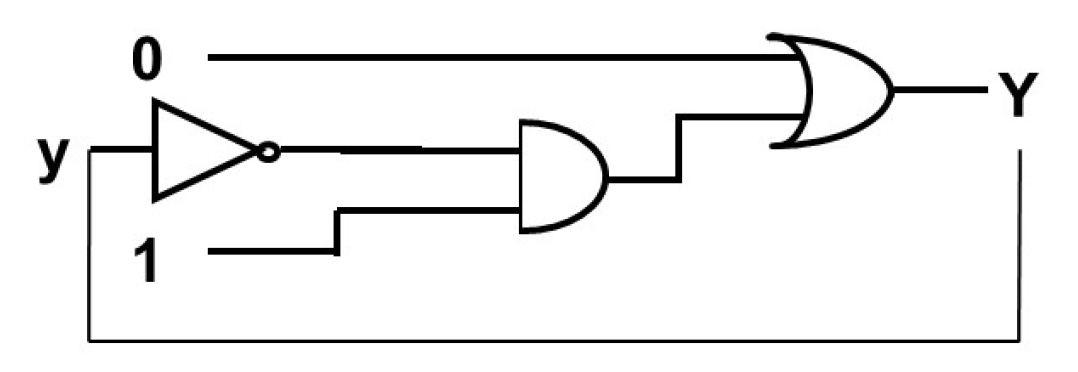
\includegraphics[height=2cm]{fig/oscillation_real.png}
        \label{subfig:oscillation_real}
    }
    \caption{环形振荡器电路图}
    \label{fig:oscillation_circuit}
\end{figure}

% 注意样例(idea/analysis 分别表示思考和分析)
\begin{note}{示波器的使用}{use_oscilloscope}
    示波器使用时需要和输入信号\textbf{共地},
    否则可能会有很大的区别(例如,不接入任何有效电压的时候可以观测到 $50\mathrm{Hz}$的信号波动),虽然由于仪器可能共用拖线板达到了共抵的效果.
\end{note}

% 代码样例
\begin{lstlisting}[language=verilog,title=tutorial\_tb.v]
initial
begin
MOV AL,100
    for (i = 0; i < 255; i = i+2)
    begin
        #50 switches=i; // time for each step
        #10 e_led = expected_led(switches); // transition time
        if (leds == e_led)
            $display ("LED output matched at", $time);
        else
            $display ("LED output mis-matched at ", $time,": expected: %b, actual: %b", e_led, leds);
    end
end
\end{lstlisting}